\documentclass{standalone}
\usepackage{tikz}
\usetikzlibrary{patterns, positioning}
\usepackage[sfdefault]{ClearSans} %% option 'sfdefault' activates Clear Sans as the default text font
\usepackage[T1]{fontenc}

\begin{document}
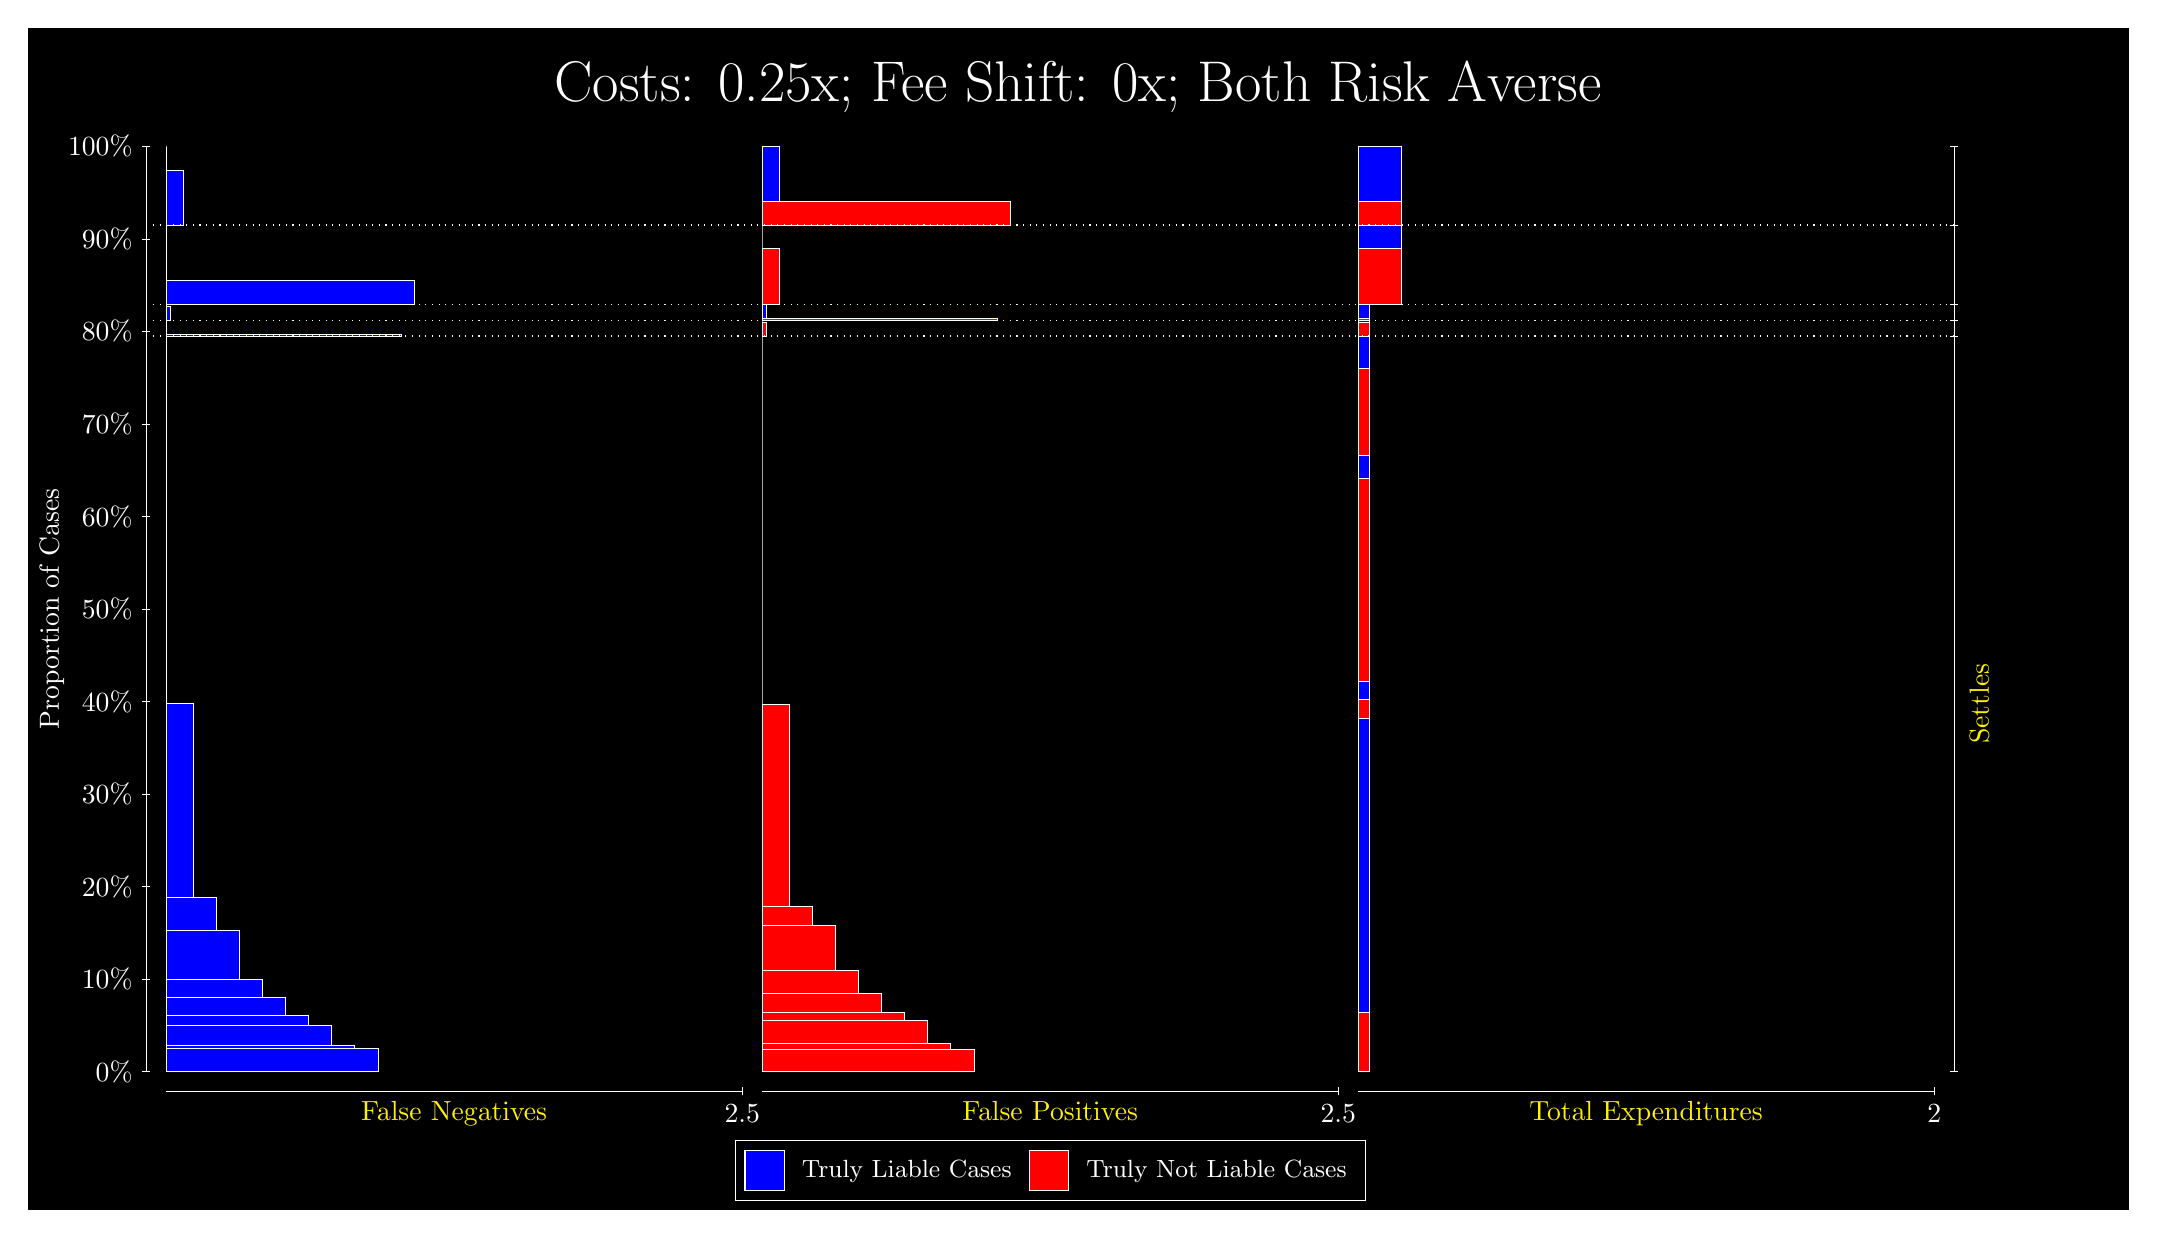
\begin{tikzpicture}
\draw[fill=black] (0,0) rectangle (26.667,15);
\draw[text=white] (0,13.5) rectangle (26.667,15) node[midway] {\huge Costs: 0.25x; Fee Shift: 0x; Both Risk Averse};
\draw[white, very thin] (1.5,1.75) -- (1.5,13.5);
\node[rotate=90, text=white, anchor=center] at (0.3, 7.625) {Proportion of Cases};
\draw[white, very thin] (1.45,1.75) -- (1.55,1.75);
\node[text=white, anchor=east] at (1.45, 1.75) {0\%};
\draw[white, very thin] (1.45,2.925) -- (1.55,2.925);
\node[text=white, anchor=east] at (1.45, 2.925) {10\%};
\draw[white, very thin] (1.45,4.1) -- (1.55,4.1);
\node[text=white, anchor=east] at (1.45, 4.1) {20\%};
\draw[white, very thin] (1.45,5.275) -- (1.55,5.275);
\node[text=white, anchor=east] at (1.45, 5.275) {30\%};
\draw[white, very thin] (1.45,6.45) -- (1.55,6.45);
\node[text=white, anchor=east] at (1.45, 6.45) {40\%};
\draw[white, very thin] (1.45,7.625) -- (1.55,7.625);
\node[text=white, anchor=east] at (1.45, 7.625) {50\%};
\draw[white, very thin] (1.45,8.8) -- (1.55,8.8);
\node[text=white, anchor=east] at (1.45, 8.8) {60\%};
\draw[white, very thin] (1.45,9.975) -- (1.55,9.975);
\node[text=white, anchor=east] at (1.45, 9.975) {70\%};
\draw[white, very thin] (1.45,11.15) -- (1.55,11.15);
\node[text=white, anchor=east] at (1.45, 11.15) {80\%};
\draw[white, very thin] (1.45,12.325) -- (1.55,12.325);
\node[text=white, anchor=east] at (1.45, 12.325) {90\%};
\draw[white, very thin] (1.45,13.5) -- (1.55,13.5);
\node[text=white, anchor=east] at (1.45, 13.5) {100\%};

\draw[white, very thin] (24.457,1.75) -- (24.457,13.5);
\draw[white, very thin] (24.407,1.75) -- (24.507,1.75);
\node[anchor=west] at (24.407, 1.75) {};
\draw[white, very thin] (24.407,11.091) -- (24.507,11.091);
\node[anchor=west] at (24.407, 11.091) {};
\draw[white, very thin] (24.407,11.293) -- (24.507,11.293);
\node[anchor=west] at (24.407, 11.293) {};
\draw[white, very thin] (24.407,11.495) -- (24.507,11.495);
\node[anchor=west] at (24.407, 11.495) {};
\draw[white, very thin] (24.407,12.501) -- (24.507,12.501);
\node[anchor=west] at (24.407, 12.501) {};
\draw[white, very thin] (24.407,13.5) -- (24.507,13.5);
\node[anchor=west] at (24.407, 13.5) {};

\draw[white, very thin, fill=blue] (1.75,1.75) rectangle (4.4397,2.0492);
\draw[white, very thin, fill=blue] (1.75,2.0492) rectangle (4.1469,2.089);
\draw[white, very thin, fill=blue] (1.75,2.089) rectangle (3.8542,2.3405);
\draw[white, very thin, fill=blue] (1.75,2.3405) rectangle (3.5614,2.4601);
\draw[white, very thin, fill=blue] (1.75,2.4601) rectangle (3.2687,2.6984);
\draw[white, very thin, fill=blue] (1.75,2.6984) rectangle (2.9759,2.9178);
\draw[white, very thin, fill=blue] (1.75,2.9178) rectangle (2.6832,3.5396);
\draw[white, very thin, fill=blue] (1.75,3.5396) rectangle (2.3904,3.9661);
\draw[white, very thin, fill=blue] (1.75,3.9661) rectangle (2.0976,6.424);
\draw[white, very thin, fill=red] (1.75,6.424) rectangle (1.75,11.091);
\draw[white, very thin, fill=blue] (1.75,11.091) rectangle (4.7324,11.114);
\draw[white, very thin, fill=red] (1.75,11.114) rectangle (1.75,11.293);
\draw[white, very thin, fill=blue] (1.75,11.293) rectangle (1.8049,11.473);
\draw[white, very thin, fill=red] (1.75,11.473) rectangle (1.75,11.495);
\draw[white, very thin, fill=blue] (1.75,11.495) rectangle (4.8971,11.797);
\draw[white, very thin, fill=red] (1.75,11.797) rectangle (1.75,12.501);
\draw[white, very thin, fill=blue] (1.75,12.501) rectangle (1.9696,13.199);
\draw[white, very thin, fill=red] (1.75,13.199) rectangle (1.75,13.5);
\draw[white, very thin, fill=red] (9.3189,1.75) rectangle (12.009,2.0274);
\draw[white, very thin, fill=red] (9.3189,2.0274) rectangle (11.716,2.1143);
\draw[white, very thin, fill=red] (9.3189,2.1143) rectangle (11.423,2.4004);
\draw[white, very thin, fill=red] (9.3189,2.4004) rectangle (11.13,2.5076);
\draw[white, very thin, fill=red] (9.3189,2.5076) rectangle (10.838,2.7459);
\draw[white, very thin, fill=red] (9.3189,2.7459) rectangle (10.545,3.0329);
\draw[white, very thin, fill=red] (9.3189,3.0329) rectangle (10.252,3.6049);
\draw[white, very thin, fill=red] (9.3189,3.6049) rectangle (9.9593,3.8486);
\draw[white, very thin, fill=red] (9.3189,3.8486) rectangle (9.6665,6.4173);
\draw[white, very thin, fill=blue] (9.3189,6.4173) rectangle (9.3189,11.091);
\draw[white, very thin, fill=red] (9.3189,11.091) rectangle (9.3738,11.271);
\draw[white, very thin, fill=blue] (9.3189,11.271) rectangle (9.3189,11.293);
\draw[white, very thin, fill=red] (9.3189,11.293) rectangle (12.301,11.316);
\draw[white, very thin, fill=blue] (9.3189,11.316) rectangle (9.3738,11.495);
\draw[white, very thin, fill=red] (9.3189,11.495) rectangle (9.5384,12.2);
\draw[white, very thin, fill=blue] (9.3189,12.2) rectangle (9.3189,12.501);
\draw[white, very thin, fill=red] (9.3189,12.501) rectangle (12.466,12.802);
\draw[white, very thin, fill=blue] (9.3189,12.802) rectangle (9.5384,13.5);
\draw[white, very thin, fill=red] (16.888,1.75) rectangle (17.025,2.5076);
\draw[white, very thin, fill=blue] (16.888,2.5076) rectangle (17.025,6.2331);
\draw[white, very thin, fill=red] (16.888,6.2331) rectangle (17.025,6.4715);
\draw[white, very thin, fill=blue] (16.888,6.4715) rectangle (17.025,6.7099);
\draw[white, very thin, fill=red] (16.888,6.7099) rectangle (17.025,9.2785);
\draw[white, very thin, fill=blue] (16.888,9.2785) rectangle (17.025,9.5777);
\draw[white, very thin, fill=red] (16.888,9.5777) rectangle (17.025,10.68);
\draw[white, very thin, fill=blue] (16.888,10.68) rectangle (17.025,11.091);
\draw[white, very thin, fill=red] (16.888,11.091) rectangle (17.025,11.271);
\draw[white, very thin, fill=blue] (16.888,11.271) rectangle (17.025,11.293);
\draw[white, very thin, fill=red] (16.888,11.293) rectangle (17.025,11.316);
\draw[white, very thin, fill=blue] (16.888,11.316) rectangle (17.025,11.495);
\draw[white, very thin, fill=red] (16.888,11.495) rectangle (17.437,12.2);
\draw[white, very thin, fill=blue] (16.888,12.2) rectangle (17.437,12.501);
\draw[white, very thin, fill=red] (16.888,12.501) rectangle (17.437,12.802);
\draw[white, very thin, fill=blue] (16.888,12.802) rectangle (17.437,13.5);
\draw[white, dotted] (1.5,11.091) -- (24.457,11.091);
\draw[white, dotted] (1.5,11.293) -- (24.457,11.293);
\draw[white, dotted] (1.5,11.495) -- (24.457,11.495);
\draw[white, dotted] (1.5,12.501) -- (24.457,12.501);
\draw[white, very thin] (1.75,1.5) -- (9.0689,1.5);
\node[text=yellow, anchor=north] at (5.4094, 1.5) {False Negatives};
\draw[white, very thin] (9.0689,1.45) -- (9.0689,1.55);
\node[text=white, anchor=north] at (9.0689, 1.45) {2.5};

\draw[white, very thin] (9.3189,1.5) -- (16.638,1.5);
\node[text=yellow, anchor=north] at (12.978, 1.5) {False Positives};
\draw[white, very thin] (16.638,1.45) -- (16.638,1.55);
\node[text=white, anchor=north] at (16.638, 1.45) {2.5};

\draw[white, very thin] (16.888,1.5) -- (24.207,1.5);
\node[text=yellow, anchor=north] at (20.547, 1.5) {Total Expenditures};
\draw[white, very thin] (24.207,1.45) -- (24.207,1.55);
\node[text=white, anchor=north] at (24.207, 1.45) {2};

\node[text=yellow, centered, rotate=90] at (24.777, 6.4206) {Settles};





\draw (12.978300999999998,1.5) node[draw=none] (baseCoordinate) {};
\begin{scope}[align=center]
        \matrix[scale=0.5, draw=white, below=0.5cm of baseCoordinate, nodes={draw}, column sep=0.1cm]{
            \node[rectangle, draw, minimum width=0.5cm, minimum height=0.5cm, fill=blue] {}; &
            \node[draw=none, font=\small, text=white] (B) {Truly Liable Cases}; &
            \node[rectangle, draw, minimum width=0.5cm, minimum height=0.5cm, fill=red] {}; &
            \node[draw=none, font=\small, text=white] (B) {Truly Not Liable Cases}; \\
            };
\end{scope}

\end{tikzpicture}
\end{document}